% Options for packages loaded elsewhere
\PassOptionsToPackage{unicode}{hyperref}
\PassOptionsToPackage{hyphens}{url}
\PassOptionsToPackage{dvipsnames,svgnames,x11names}{xcolor}
%
\documentclass[
  letterpaper,
  DIV=11,
  numbers=noendperiod]{scrreprt}

\usepackage{amsmath,amssymb}
\usepackage{iftex}
\ifPDFTeX
  \usepackage[T1]{fontenc}
  \usepackage[utf8]{inputenc}
  \usepackage{textcomp} % provide euro and other symbols
\else % if luatex or xetex
  \usepackage{unicode-math}
  \defaultfontfeatures{Scale=MatchLowercase}
  \defaultfontfeatures[\rmfamily]{Ligatures=TeX,Scale=1}
\fi
\usepackage{lmodern}
\ifPDFTeX\else  
    % xetex/luatex font selection
\fi
% Use upquote if available, for straight quotes in verbatim environments
\IfFileExists{upquote.sty}{\usepackage{upquote}}{}
\IfFileExists{microtype.sty}{% use microtype if available
  \usepackage[]{microtype}
  \UseMicrotypeSet[protrusion]{basicmath} % disable protrusion for tt fonts
}{}
\makeatletter
\@ifundefined{KOMAClassName}{% if non-KOMA class
  \IfFileExists{parskip.sty}{%
    \usepackage{parskip}
  }{% else
    \setlength{\parindent}{0pt}
    \setlength{\parskip}{6pt plus 2pt minus 1pt}}
}{% if KOMA class
  \KOMAoptions{parskip=half}}
\makeatother
\usepackage{xcolor}
\usepackage[heightrounded]{geometry}
\setlength{\emergencystretch}{3em} % prevent overfull lines
\setcounter{secnumdepth}{-\maxdimen} % remove section numbering
% Make \paragraph and \subparagraph free-standing
\ifx\paragraph\undefined\else
  \let\oldparagraph\paragraph
  \renewcommand{\paragraph}[1]{\oldparagraph{#1}\mbox{}}
\fi
\ifx\subparagraph\undefined\else
  \let\oldsubparagraph\subparagraph
  \renewcommand{\subparagraph}[1]{\oldsubparagraph{#1}\mbox{}}
\fi


\providecommand{\tightlist}{%
  \setlength{\itemsep}{0pt}\setlength{\parskip}{0pt}}\usepackage{longtable,booktabs,array}
\usepackage{calc} % for calculating minipage widths
% Correct order of tables after \paragraph or \subparagraph
\usepackage{etoolbox}
\makeatletter
\patchcmd\longtable{\par}{\if@noskipsec\mbox{}\fi\par}{}{}
\makeatother
% Allow footnotes in longtable head/foot
\IfFileExists{footnotehyper.sty}{\usepackage{footnotehyper}}{\usepackage{footnote}}
\makesavenoteenv{longtable}
\usepackage{graphicx}
\makeatletter
\def\maxwidth{\ifdim\Gin@nat@width>\linewidth\linewidth\else\Gin@nat@width\fi}
\def\maxheight{\ifdim\Gin@nat@height>\textheight\textheight\else\Gin@nat@height\fi}
\makeatother
% Scale images if necessary, so that they will not overflow the page
% margins by default, and it is still possible to overwrite the defaults
% using explicit options in \includegraphics[width, height, ...]{}
\setkeys{Gin}{width=\maxwidth,height=\maxheight,keepaspectratio}
% Set default figure placement to htbp
\makeatletter
\def\fps@figure{htbp}
\makeatother

\usepackage{fvextra}
\DefineVerbatimEnvironment{Highlighting}{Verbatim}{breaklines,commandchars=\\\{\}}
\KOMAoption{captions}{tableheading}
\makeatletter
\@ifpackageloaded{caption}{}{\usepackage{caption}}
\AtBeginDocument{%
\ifdefined\contentsname
  \renewcommand*\contentsname{Table of contents}
\else
  \newcommand\contentsname{Table of contents}
\fi
\ifdefined\listfigurename
  \renewcommand*\listfigurename{List of Figures}
\else
  \newcommand\listfigurename{List of Figures}
\fi
\ifdefined\listtablename
  \renewcommand*\listtablename{List of Tables}
\else
  \newcommand\listtablename{List of Tables}
\fi
\ifdefined\figurename
  \renewcommand*\figurename{Figure}
\else
  \newcommand\figurename{Figure}
\fi
\ifdefined\tablename
  \renewcommand*\tablename{Table}
\else
  \newcommand\tablename{Table}
\fi
}
\@ifpackageloaded{float}{}{\usepackage{float}}
\floatstyle{ruled}
\@ifundefined{c@chapter}{\newfloat{codelisting}{h}{lop}}{\newfloat{codelisting}{h}{lop}[chapter]}
\floatname{codelisting}{Listing}
\newcommand*\listoflistings{\listof{codelisting}{List of Listings}}
\makeatother
\makeatletter
\makeatother
\makeatletter
\@ifpackageloaded{caption}{}{\usepackage{caption}}
\@ifpackageloaded{subcaption}{}{\usepackage{subcaption}}
\makeatother
\makeatletter
\@ifpackageloaded{tcolorbox}{}{\usepackage[skins,breakable]{tcolorbox}}
\makeatother
\makeatletter
\@ifundefined{shadecolor}{\definecolor{shadecolor}{rgb}{.97, .97, .97}}{}
\makeatother
\makeatletter
\@ifundefined{codebgcolor}{\definecolor{codebgcolor}{HTML}{D3D3D3}}{}
\makeatother
\makeatletter
\ifdefined\Shaded\renewenvironment{Shaded}{\begin{tcolorbox}[enhanced, breakable, frame hidden, colback={codebgcolor}, sharp corners, boxrule=0pt]}{\end{tcolorbox}}\fi
\makeatother
\ifLuaTeX
  \usepackage{selnolig}  % disable illegal ligatures
\fi
\usepackage{bookmark}

\IfFileExists{xurl.sty}{\usepackage{xurl}}{} % add URL line breaks if available
\urlstyle{same} % disable monospaced font for URLs
\hypersetup{
  colorlinks=true,
  linkcolor={blue},
  filecolor={Maroon},
  citecolor={Blue},
  urlcolor={Blue},
  pdfcreator={LaTeX via pandoc}}

\author{}
\date{}

\begin{document}

\RecustomVerbatimEnvironment{verbatim}{Verbatim}{
  showspaces = false,
  showtabs = false,
  breaksymbolleft={},
  breaklines
}

\renewcommand*\contentsname{Table of contents}
{
\hypersetup{linkcolor=}
\setcounter{tocdepth}{1}
\tableofcontents
}
\section{An example notebook}\label{an-example-notebook}

If you want to see an example for documented code, check out
\href{https://github.com/ndombrowski/cli_workshop/tree/main/example_doc}{an
example} for how I might have recorded how I analysed some sequence data
myself.

The link above leads you to an example for:

\begin{itemize}
\tightlist
\item
  How could I use github to make my code available to others
\item
  How could a ``code book'' look like? The example you see in the folder
  is provided a Quarto markdown file
  \href{https://github.com/ndombrowski/cli_workshop/blob/main/example_doc/example_notebook.qmd}{here}
  and for convenience the report was also rendered as a
  \href{https://github.com/ndombrowski/cli_workshop/blob/main/docs/example_doc/example_notebook.html}{html}
  to make it easier to read for potential collaborators. To view the
  HTML report, you need to download it first.
\end{itemize}

The example is based on the data you analyse throughout this tutorial,
so the actual code might only make sense after you have finished the
tutorial. Feel free to revisit this page after you have written some
code yourself.

Please note that this is just an example to get you started and such a
report might look different depending on your needs.

Below you find some general hints for what to put into different
sections that you can see in the qmd file.

\subsection{YAML headers}\label{yaml-headers}

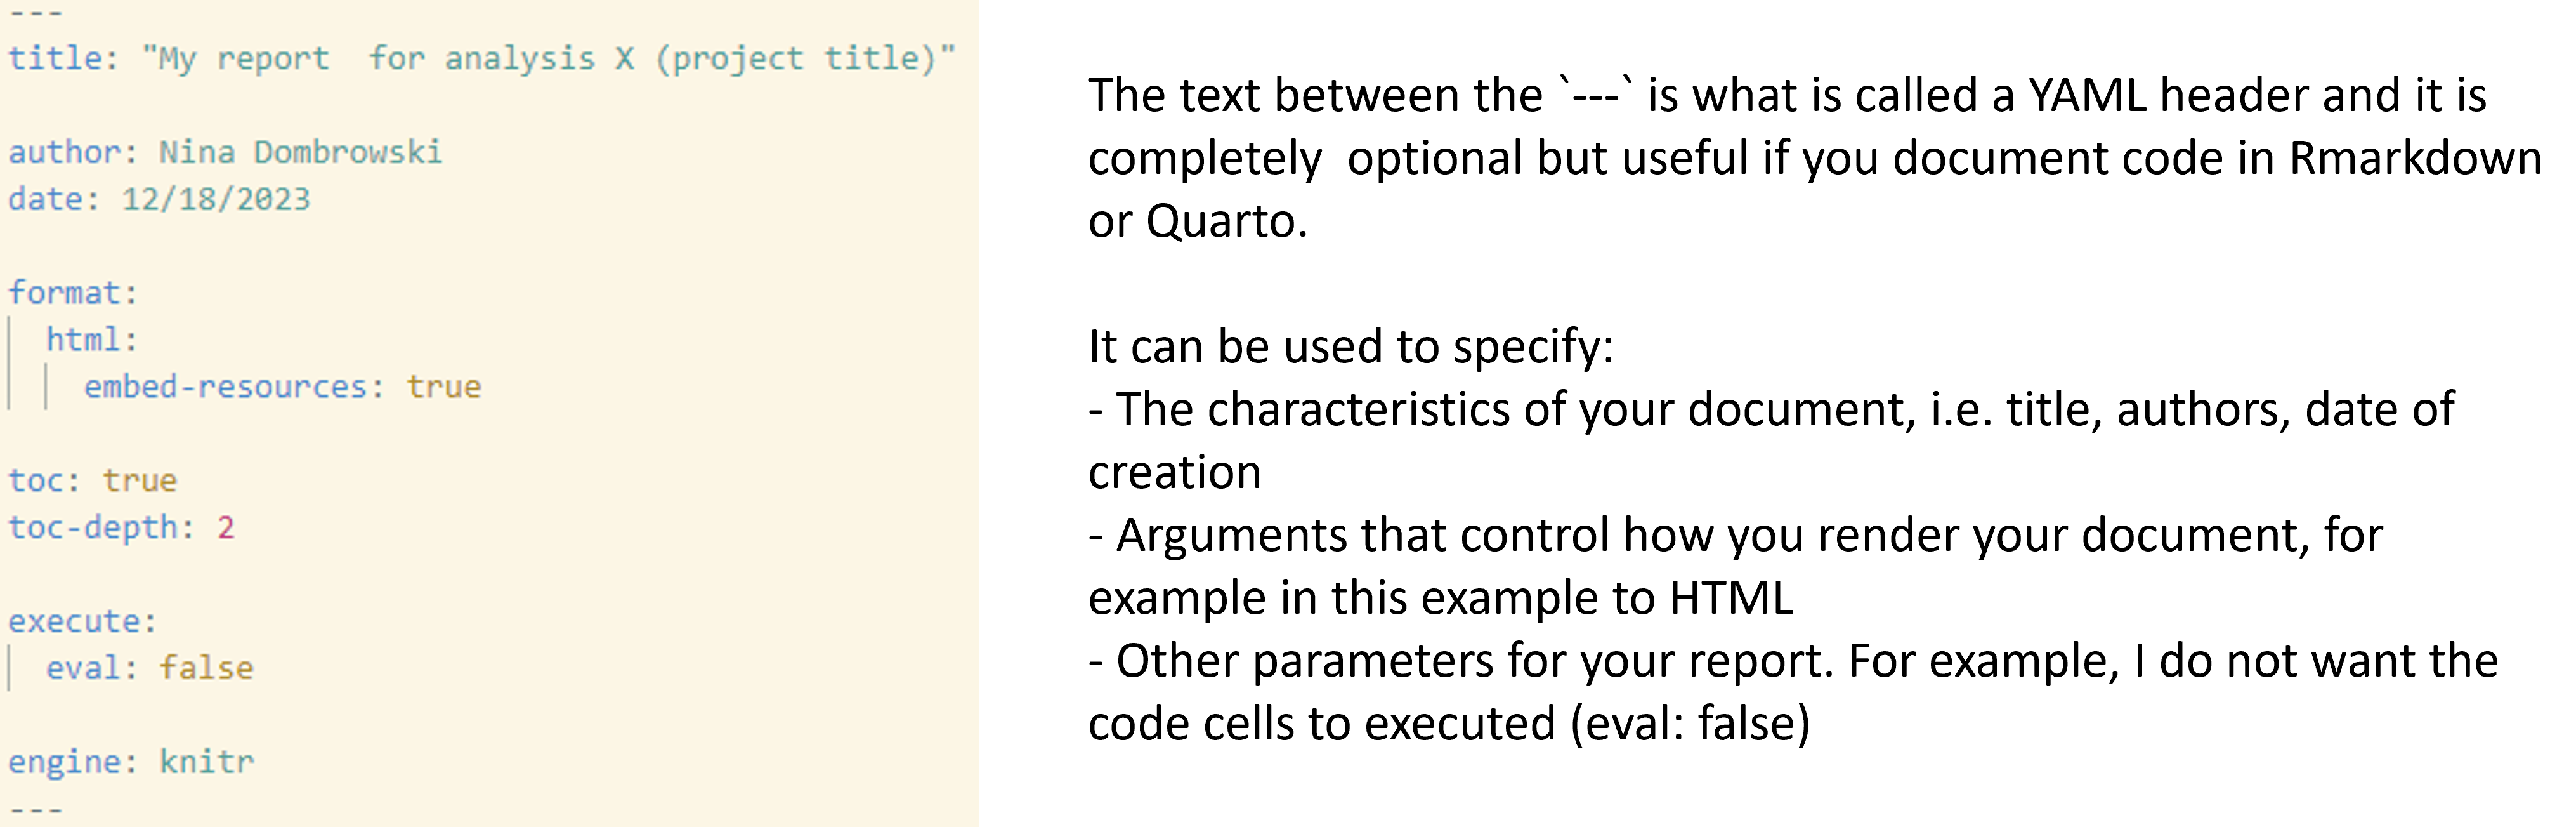
\includegraphics[width=7.84375in,height=\textheight]{../img/yaml_header.png}

\subsection{Setting up your working
directory}\label{setting-up-your-working-directory}

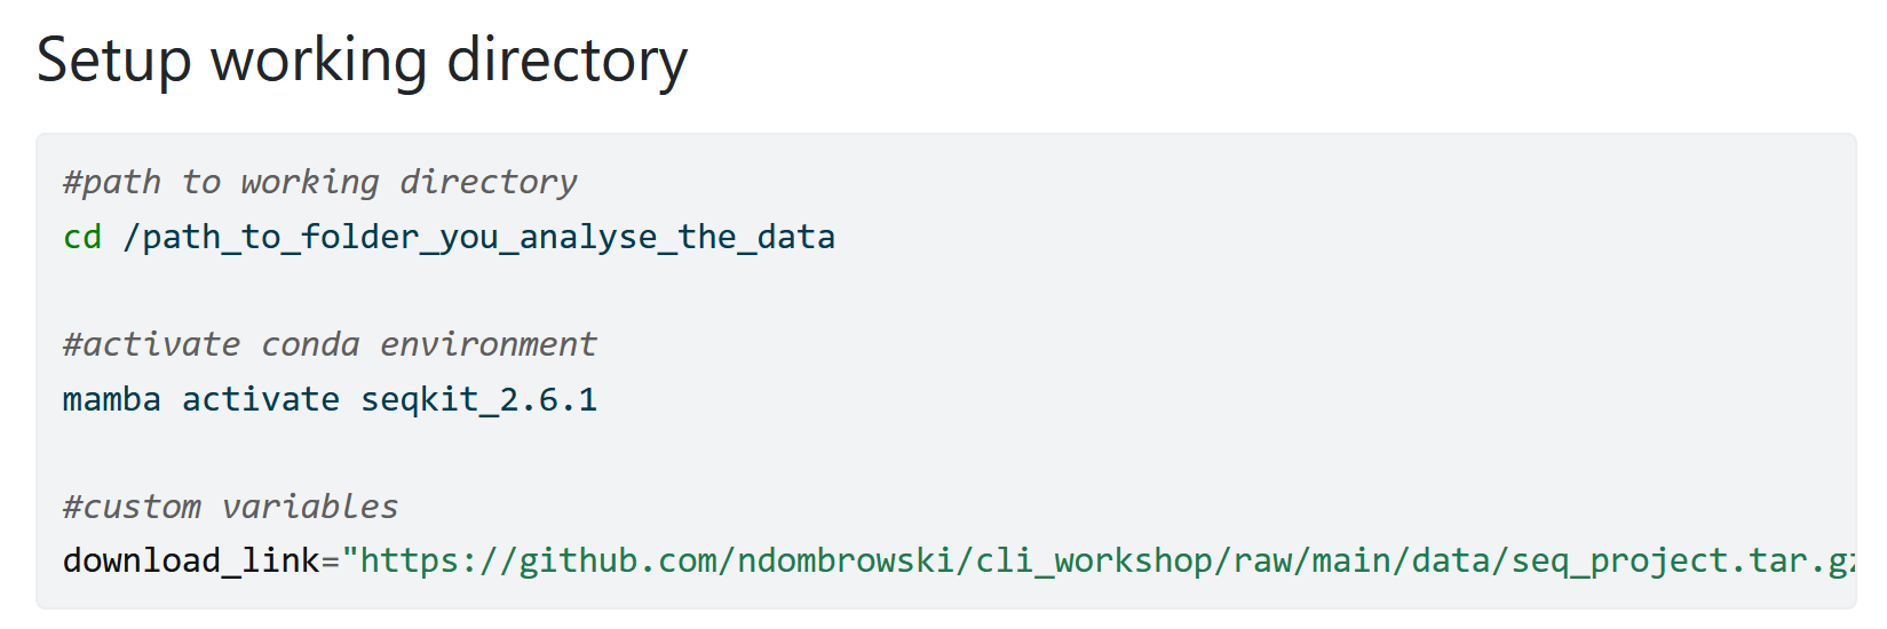
\includegraphics[width=5.71875in,height=\textheight]{../img/general_setup.png}

In this first section I add everything that a user that wants to use my
workflow has to change and I try to standardize the code below, so that
another user could just run this as is without having to edit anything.
Typically things to add are:

\begin{itemize}
\tightlist
\item
  From where to start the analyses
\item
  Custom paths, to for example for databases that need to be downloaded
  from elsewhere
\item
  Custom variables: In the example above I store the link to the data in
  a variable called \texttt{download\_link}, I then use the variable in
  the code below to download the data. By doing it this way I have one
  location in the code another person needs to change the code when for
  example the path to the data changes. The code below stays the same.
  When writing code try to think ahead and minimize the number of
  instances where things need to be changed if for example the location
  to your data changes.
\item
  \ldots{}
\end{itemize}

I tend to NOT add the information how I use \texttt{scp} to log into an
HPC to keep my user name and login information private.

\subsection{Sanity checks}\label{sanity-checks}

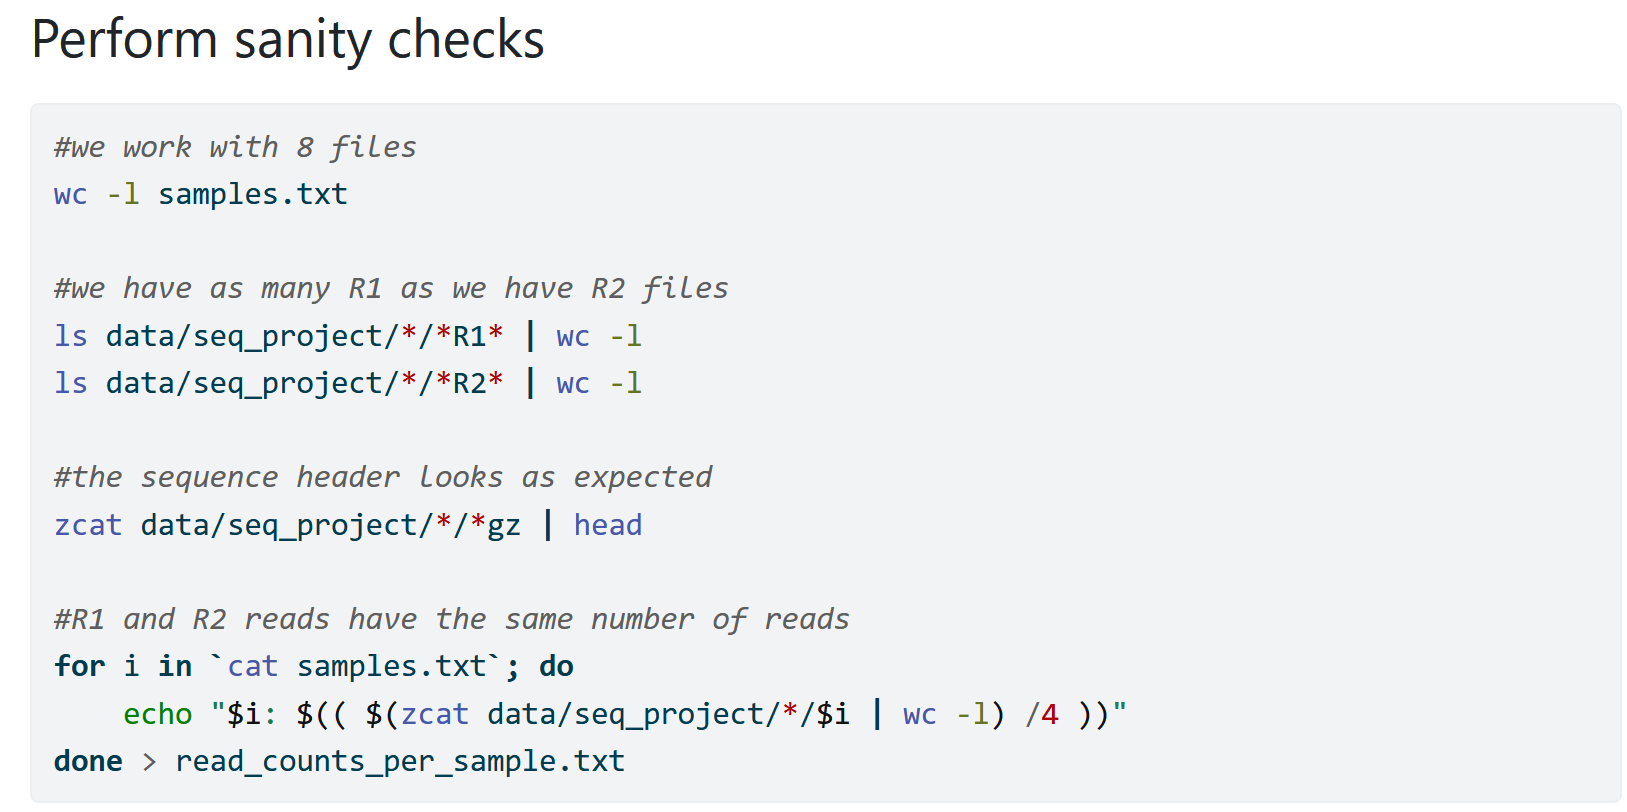
\includegraphics[width=5.84375in,height=\textheight]{../img/sanity_check.png}

When I first start working with new data, I try to add as many sanity
checks as possible to ensure that my data looks good. That way I avoid
that I don't notice an issue and run into trouble further down the line.
I at the same time understand my data more and learn with how many
samples and how much data I am working with.

I also add such sanity checks whenever I modify my data. For example,
when I merge individual files into a large file I might count the lines
for the individual files and the combined file simply to ensure that I
used my wildcards correctly.

Remember: The computer is only as smart as the person using it and will
blindly run your commands. Because of that the computer can do
unexpected things and you need to account for that.

\subsection{Using markdown to make
notes}\label{using-markdown-to-make-notes}

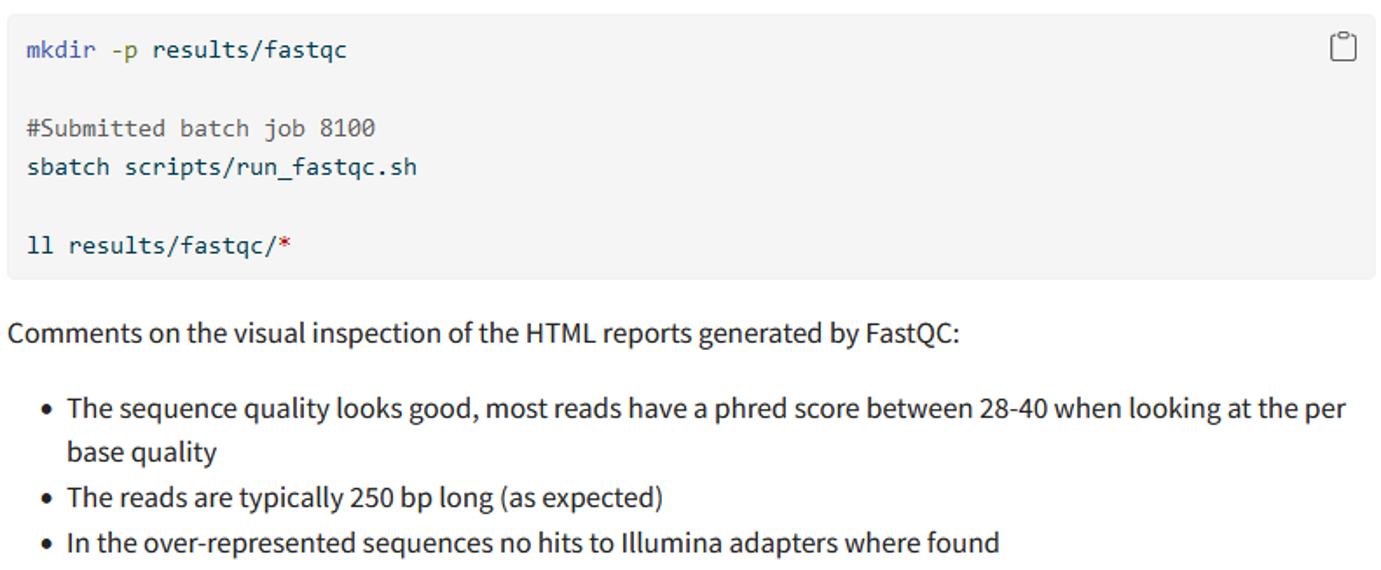
\includegraphics[width=5.65625in,height=\textheight]{../img/comments_in_code.png}

In the example above I use markdown to not only document my code but
also add some comments whenever I might need it. For example here, I
added some notes about what the results from FastQC actually told me.

This kind of documentation can be useful for:

\begin{itemize}
\item
  Justifying decisions further down the line. In this example, I might
  decide on how to clean the sequencing data. For example, if I would
  have found a lot of low quality reads or the adapter still being part
  of the sequence then I would have specifically cleaned my sequences to
  deal with that
\item
  Future you. If you read the report a month, or a year, later you have
  the key information in your report and don't have to open the HTML
  reports again.
\end{itemize}

\subsection{Documenting external
scripts}\label{documenting-external-scripts}

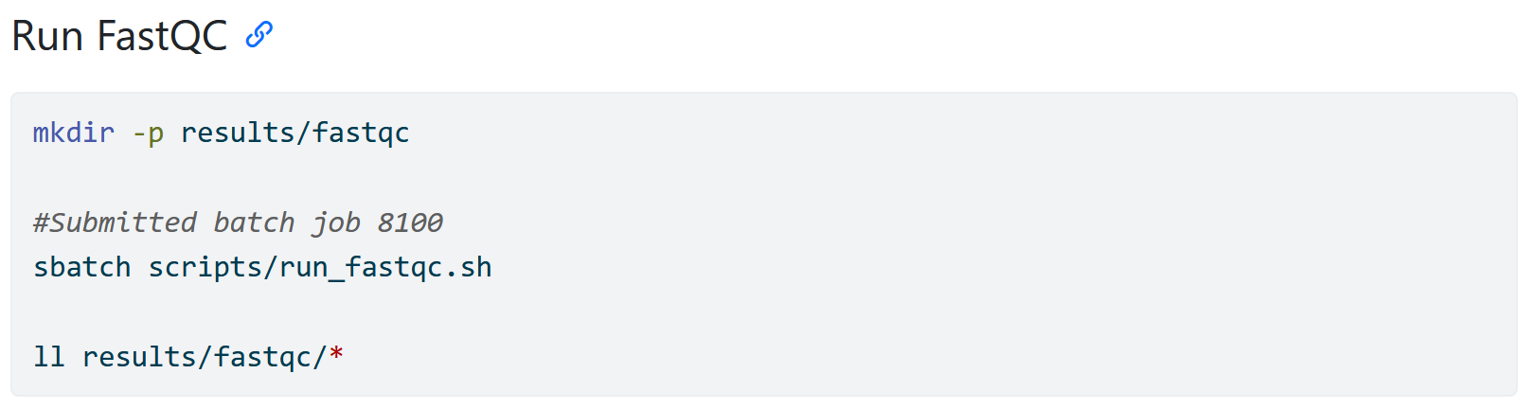
\includegraphics[width=5.82292in,height=\textheight]{../img/external_scripts.png}

This part might make more sense after you have worked through the part
of the tutorial about using an HPC. But what you see here is how I have
written down code that simply says that I submitted a script to a HPC
but it does not actually say how I ran the FastQC software. The actual
code is ``hidden'' inside of the run\_fastqc.sh script. This also means
that a person reading your workflow does not have the code right away.
You can deal with this in two ways.

\begin{enumerate}
\def\labelenumi{\arabic{enumi}.}
\tightlist
\item
  Instead of the sbatch command, you can add the actual line of code
  that was run on the compute node.
\item
  When publishing your code with your manuscript, add the whole scripts
  folder to where you publish the main code, i.e.~on
  \href{https://github.com/ndombrowski/cli_workshop/tree/main/example_doc}{github}
  or \href{https://zenodo.org/records/3839790}{zenodo}
\end{enumerate}

I tend to prefer number 2 because I like to record the code in my
notebooks exactly as I ran them but you can do it differently as long as
all the code you ran is recorded and accessible to others once you
publish your data.



\end{document}
